\documentclass[11pt]{article}

\usepackage{nmrdoc}
\usepackage{siunitx}
\usepackage{bm}
\usepackage{tikz}

\sisetup{per-mode=symbol}
\DeclareSIUnit{\angstrom}{\text{\AA}}
\DeclareSIUnit{\ppm}{ppm}
\DeclareSIUnit{\elementarycharge}{e}

\newcommand{\code}[1]{\texttt{#1}}
\newcommand{\dd}{\,d}
\newcommand{\doi}[1]{\href{https://doi.org/#1}{\nolinkurl{#1}}}

\setlength{\parindent}{0pt}
\setlength{\parskip}{0.48em}
\emergencystretch=5em
\AtBeginDocument{\raggedright}

\begin{document}
\NmrTitle{Method and Proxy: The Shape of Each Tool's Question}
\tableofcontents
\clearpage

\section{What Proxy Means Here}

The companion on physics architecture names the hidden object: Ramsey nuclear
magnetic shielding, the electronic current response to an applied field and a
nuclear magnetic moment \cite{ramsey1950,facelli2011}. The companion on
categorical grounding names the empirical world in which the object is seen:
amide protons report hydrogen bonds and electric fields; aromatic-near protons
report ring currents; backbone carbons report peptide geometry; side-chain atoms
report rotamers, contacts, and solvent exposure. This document names the shape
of the tools between those two views.

``Direct expression of the physics'' usually means ``exact maths on a proxied
source.'' The maths can be exact: Biot--Savart gives the exact field of a
current loop; the electric-field gradient is the exact second derivative of a
point-charge potential; the dipolar kernel is the exact field shape of a point
magnetic dipole. The proxy is not in the arithmetic. It is in what the
arithmetic acts on. It is forced by computability: the code cannot integrate the
true quantum current density of a protein frame, so it substitutes a source the
maths can chew. That substitution is the proxy, baked into the technique, not
bolted on afterward.

The geometric kernel is therefore the question the tool poses to the universe.
Calibration is how we listen for the answer. A kernel says, for example:
if this bond's anisotropy is placed at its midpoint, is this the angular and
distance pattern carried by the shielding data? If this aromatic ring is
replaced by a pair of current loops, does the DFT shielding respond along that
shape? If this hydrogen bond is summarized by a local table indexed by
\((r,\theta,\rho)\), does that table carry the local electronic reorganization?
The proxy is the form of the question.

The recurring vocabulary is small:

\textbf{The master proxy} is the classical source standing in for a quantum
response. A current loop, point susceptibility, point charge, quadrupole, or
contact tensor carries the geometry of an effect. The coefficient that would
make it a shielding contribution --- \(\Delta\chi\), a ring-current intensity,
Buckingham's \(A\) or \(\gamma\), a quadrupole strength, \(C_6\), or a fitted
hydrogen-bond coefficient --- is the part still to be learned.

\textbf{Source-shape proxies} collapse extended objects to compact ones.
McConnell places a distributed bond anisotropy at a midpoint.
RingSusceptibility places a whole aromatic ring at a point. PiQuadrupole places
an aromatic \(\pi\) distribution at a point axial quadrupole. What changes is
not the law applied to the source; it is the shape of the source offered to the
law.

\textbf{Magnitude and convention proxies} hold scale still so shape can be read.
BiotSavart uses \(\SI{1}{\nano\ampere}\). Dispersion sets \(C_6=1\).
McConnell and RingSusceptibility use unit source weights. Johnson--Bovey lobe
offsets are fixed by ring type. These choices make the raw feature a measured
shape, not a completed shielding.

\textbf{Discretization proxies} trade continuity for computable samples:
polygon loops for smooth aromatic current paths, fan triangles and seven-point
cubature for ring surfaces, trilinear interpolation for potential and DFT grids,
and central differences for derivatives of a stored scalar potential.

\textbf{Model-substitution proxies} replace an inaccessible source by a
computable model of it: Poisson--Boltzmann continuum electrostatics for a
solvated protein environment, fixed three-site water charges for explicit
solvent electron density, EEQ charges for the real ground-state charge
distribution, and Larsen donor/acceptor archives for hydrogen-bond chemistry.

These are not ranks of blame. They are names for how method reaches toward
physics.

\section{The Literal--to--Borrowed Spine}

The spectrum that matters is how literal the source is, not how exact the
arithmetic is. At the literal end, BiotSavart really computes the magnetic
field of a current, although the ring current itself has been turned into two
unit-current polygon loops. Near it, WaterField really computes fields and
field gradients from point charges, and Haigh--Mallion really integrates a
dipolar kernel over a ring surface. In the middle, McConnell and
RingSusceptibility use real dipolar angular physics after collapsing an
extended anisotropy to a point. Farther along, Dispersion borrows the rank-2
angular shape but changes the distance law to \(r^{-6}\), and HBond borrows the
same McConnell tensor as a way to ask whether a chemically real hydrogen-bond
axis carries shielding. At the contextual edge, HydrationShell emits solvent
arrangement rather than a field or tensor. LarsenHBond is the special case: its
source is already DFT shielding data, so its proxy lies in classing,
interpolation, and local scope, not in a borrowed geometric kernel.

\begin{center}
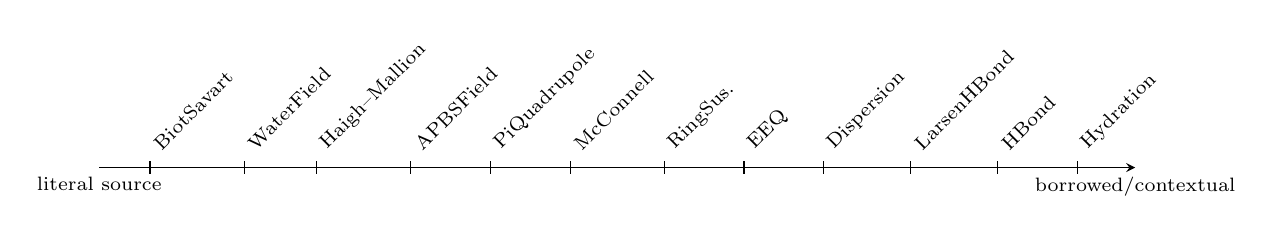
\begin{tikzpicture}[x=0.92cm,y=1.0cm,line width=0.45pt,>=stealth]
  \draw[->] (0,0) -- (14.3,0);
  \node[below] at (0,0) {\scriptsize literal source};
  \node[below] at (14.3,0) {\scriptsize borrowed/contextual};

  \foreach \x/\lab in {
    0.7/BiotSavart,
    2.0/WaterField,
    3.0/Haigh--Mallion,
    4.3/APBSField,
    5.4/PiQuadrupole,
    6.5/McConnell,
    7.8/RingSus.,
    8.9/EEQ,
    10.0/Dispersion,
    11.2/LarsenHBond,
    12.4/HBond,
    13.5/Hydration}
  {
    \draw (\x,0.08) -- (\x,-0.08);
    \node[rotate=45,anchor=west] at (\x,0.18) {\scriptsize \lab};
  }
\end{tikzpicture}
\end{center}

This line is not a scorecard. It is a reading order. Moving right does not make
the method less useful; it changes what the method is asking. A literal current
loop asks for a magnetic field. A hydrogen-bond axis asks whether a strong local
chemical direction can carry a shielding response after calibration. A
hydration half-shell asks whether the local solvent arrangement conditions the
same response.

\section{The Shared Kernel as Question}

Most tools return to the Hessian of \(1/\rho\),
\[
  D_{ab}(\bm\rho)
  =
  \frac{3\rho_a\rho_b-\delta_{ab}\rho^2}{\rho^5}
  =
  \frac{3\hat\rho_a\hat\rho_b-\delta_{ab}}{\rho^3}.
\]
\(\bm\rho\) is the displacement from a source point to the observed atom,
\(\rho=|\bm\rho|\), and \(\delta_{ab}\) is one when the Cartesian directions
\(a\) and \(b\) are the same. The tensor is symmetric and traceless. Along the
line of sight it has eigenvalue \(+2/\rho^3\); in the two perpendicular
directions it has \(-1/\rho^3\). The three values sum to zero.

That one tensor is both a magnetic and an electric object. In magnetostatics it
is the angular field shape of a point dipole. In electrostatics it is the
electric-field gradient of a point charge away from the charge. In McConnell,
RingSusceptibility, and HBond it is folded into an asymmetric susceptibility
kernel whose trace average is
\[
  f(\bm\rho,\hat{\bm u})
  =
  \frac{3(\hat{\bm\rho}\cdot\hat{\bm u})^2-1}{\rho^3}.
\]
\(\hat{\bm u}\) is the source axis: a bond direction, a ring normal, or an
\(N\cdots O\) hydrogen-bond axis. In Dispersion the same angular matrix is kept
but the distance law becomes \(r^{-6}\). In PiQuadrupole the \(1/r\) source law
is differentiated two steps farther. The repeated form is not accidental. It is
the common grammar by which these classical sources ask about a rank-2
shielding response.

\section{Bond and Ring Susceptibility Proxies}

\subsection{McConnell}

McConnell asks: if a covalent bond is an anisotropic magnetic object, what
rank-2 shape does that bond cast at a nearby nucleus? The physical reach is
bond and group anisotropy, especially peptide \(C=O\), peptide \(C-N\),
side-chain carbonyls, aromatic bonds, and other covalent axes that move when
backbone and side-chain geometry move \cite{mcconnell1957,dedios1993}.

The code's source is a bond midpoint \(\bm m\), a bond length \(\ell\), and a
unit bond axis \(\hat{\bm b}\). For an atom at \(\bm r\),
\(\bm x=\bm r-\bm m\), \(r=|\bm x|\),
\(\hat{\bm d}=\bm x/r\), and
\(c=\hat{\bm d}\cdot\hat{\bm b}\). The full per-bond tensor is
\[
  M_{ab}
  =
  \frac{
    9c\,\hat d_a\hat b_b
    -3\hat b_a\hat b_b
    -\left(3\hat d_a\hat d_b-\delta_{ab}\right)}
  {r^3}.
\]
The scalar \(f=(3c^2-1)/r^3\) is the trace average of this full tensor for a
nondegenerate bond. The asymmetric first dyad can populate \(T_1\); the
symmetric traceless remainder populates \(T_2\).

The proxy is source-shape and magnitude at once. A bond is not a point; its
electron density and susceptibility anisotropy are distributed along an
extended covalent region. McConnell collapses that distribution to the midpoint
and asks the dipolar law to speak from there. The calculator also assigns unit
weight. It does not multiply by a bond-specific \(\Delta\chi\), so the shape is
computed and the material strength is left for calibration.

Its numerical guards also express the source-shape proxy. The atom path omits a
target closer than half the bond length to the midpoint, because inside that
ball the midpoint no longer stands cleanly for the extended bond. The singular
guard at \(\SI{0.1}{\angstrom}\), the self-source filter, and the
\(\SI{10}{\angstrom}\) midpoint query decide membership in the question; they
do not taper or rescale accepted terms.

On the spectrum, McConnell is middle. The angular law is physical and old. The
point midpoint, unit bond weight, and missing \(\Delta\chi\) are the proxy.
The tool reaches toward anisotropic covalent shielding in the atom categories
where local bond geometry is one of the real determinants.

\subsection{RingSusceptibility}

RingSusceptibility asks: if the aromatic ring were a single anisotropic
susceptibility at its centre, with its principal axis along the fitted normal,
what inverse-cube tensor would reach the atom? It takes the McConnell question
and replaces the bond axis \(\hat{\bm b}\) by the ring normal
\(\hat{\bm n}\). With \(\bm x=\bm r-\bm c\), \(r=|\bm x|\),
\(\hat{\bm d}=\bm x/r\), and \(u=\hat{\bm d}\cdot\hat{\bm n}\), the scalar is
\[
  f_{\mathrm{ring}}=\frac{3u^2-1}{r^3},
\]
and the full tensor is the same three-term \(M_{ab}\) with
\(\hat{\bm b}\mapsto\hat{\bm n}\).

The proxy is a strong source-shape compression. The ring's \(\pi\) system has
extent, vertices, height above the plane, and a current path. This calculator
keeps the centre and the normal, obtained from the shared SVD ring geometry,
and asks only the far-field point-susceptibility question. It does not multiply
by a ring-current intensity, a ring-type susceptibility, a Johnson--Bovey lobe
offset, or a fitted scale. All accepted rings carry unit geometric weight.

The near-field exclusion is therefore meaningful. A target inside the mean ring
radius is not being asked of the point-source proxy on the atom path; ring
vertices and their bonded neighbours are also omitted because they belong to a
through-bond aromatic regime rather than a through-space ring-source regime.
The accepted tensor is decomposed raw, so the \(T_0\), \(T_1\), and \(T_2\)
channels retain the complete point-susceptibility question.

On the spectrum, RingSusceptibility sits just beyond McConnell. It uses the
same literal dipolar angular law, but the source it compresses is a whole
aromatic ring rather than one bond. It reaches toward the ring-current and
ring-susceptibility category for aromatic-proximal nuclei, especially protons
whose shifts have long required explicit aromatic terms
\cite{pople1956,case1995,christensen2011}.

\section{Aromatic Ring-Current Proxies}

\subsection{BiotSavart}

BiotSavart asks the most literal magnetic question in the suite: what secondary
magnetic field would a circulating aromatic current create at the atom? For a
current \(I\) flowing along a curve, the field is
\[
  \bm B(\bm r)
  =
  \frac{\mu_0 I}{4\pi}
  \oint
  \frac{\dd\bm\ell\times(\bm r-\bm s)}
       {|\bm r-\bm s|^3}.
\]
\(\dd\bm\ell\) is a directed element of the current path at source point
\(\bm s\). \(\bm r-\bm s\) points from that current element to the field point.
The cross product supplies the curling direction of the magnetic field.

The code does not integrate over a smooth quantum current density. It replaces
the aromatic current by the Johnson--Bovey double loop: two polygonal copies of
the ring, displaced by a fixed ring-type lobe offset on either side of the
fitted ring plane \cite{johnson1958}. Each lobe carries half the requested
current. Each polygon edge is a straight wire segment, and the segment field is
evaluated by the closed-form finite-wire Biot--Savart expression, not by
quadrature.

The magnitude proxy is explicit. Atom calculations call the double-loop field
with \(\SI{1}{\nano\ampere}\). The code records the ring intensity as
provenance but does not multiply it into the tensor. The shielding-like matrix
is
\[
  G_{ab}=-10^6 B_a^{(1)} n_b .
\]
\(B_a^{(1)}\) is component \(a\) of the unit-current field, and \(n_b\) is
component \(b\) of the ring normal. The column index says only the applied-field
component normal to the ring drives this current in the model. The row index is
the secondary-field component produced at the atom. The outer product has rank
at most one and can be asymmetric.

On the spectrum, BiotSavart is closest to literal. Its arithmetic is the real
field law of a current. The proxies are the current source itself: polygon
loops for the unknown quantum current path, fixed lobe offsets for the two
\(\pi\) lobes, and unit current for uncalibrated strength. It reaches toward the
aromatic ring-current shielding term named by Pople, Johnson--Bovey, and later
protein calibrations \cite{pople1956,johnson1958,case1995,boyd2002}.

\subsection{Haigh--Mallion}

Haigh--Mallion asks: what field-like tensor is obtained if the aromatic ring
interior is read as a surface of dipolar response? The raw object is
\[
  H_{ab}(\bm r)
  =
  \int_S
  \left(
    \frac{3\rho_a\rho_b}{\rho^5}
    -\frac{\delta_{ab}}{\rho^3}
  \right)
  \dd S .
\]
\(S\) is the fan-triangulated ring surface, \(\dd S\) is an area element, and
\(\bm\rho=\bm r-\bm s\) points from a surface point \(\bm s\) to the atom. The
integrand is the same dipolar kernel. The reported kernel contracts the surface
tensor with the ring normal and forms
\[
  V_a=H_{ab}n_b,
  \qquad
  G_{ab}=-V_a n_b .
\]

The proxy is neither a current wire nor a point susceptibility. It is a surface
reading of the ring response, inherited from the Haigh--Mallion lineage
\cite{haigh1979}. The ring interior is not flattened onto the fitted plane; the
fan uses the actual ring centre and vertices. But continuity is traded for
tractable quadrature. Each fan triangle receives a seven-point degree-five
rule, with depth-two adaptive subdivision near the target. Degenerate triangles
and near-singular quadrature points are omitted rather than repaired by a
different source.

The magnitude proxy is again the absence of the electronic response
coefficient. The surface integral carries the geometry and the normal
projection; calibration must decide the scale. The raw \(\bm H\) is symmetric
and traceless in exact arithmetic because it integrates symmetric traceless
kernels. The reported \(\bm G\), after normal contraction and outer product,
can populate all three \(T_0/T_1/T_2\) channels.

On the spectrum, Haigh--Mallion is close but less literal than BiotSavart. It
does not compute the field of a current path. It asks a surface-kernel version
of the same aromatic response question, retaining ring extent more richly than
RingSusceptibility and leaving strength for calibration.

\section{Electrostatic and Multipole Proxies}

\subsection{APBSField}

APBSField asks: what electric field and electric-field-gradient tensor does a
continuum electrostatic model assign to each atom in this conformation? The
physics bridge is Buckingham's expansion: shielding can change with local
electric fields and field gradients, with coefficients that depend on the
nucleus and local electronic structure \cite{buckingham1960,hass2008,kukic2013}.

The source proxy is model substitution. APBS solves a linearized
Poisson--Boltzmann problem for a solvated biomolecule on a grid
\cite{baker2001}. The calculator receives only the scalar potential
\(\phi\), in APBS units. It does not receive APBS-internal fields. At an atom
\(\bm r_i\), it forms a central finite difference,
\[
  E_a(\bm r_i)
  =
  -\frac{\phi(\bm r_i+h_a\hat{\bm e}_a)
          -\phi(\bm r_i-h_a\hat{\bm e}_a)}
         {2h_a}.
\]
\(h_a\) is the grid spacing along axis \(a\), and
\(\hat{\bm e}_a\) is the Cartesian unit vector. The minus sign is
\(\bm E=-\nabla\phi\). The field-gradient entry is then another central
difference,
\[
  G_{ab}(\bm r_i)
  =
  \frac{E_a(\bm r_i+h_b\hat{\bm e}_b)
        -E_a(\bm r_i-h_b\hat{\bm e}_b)}
       {2h_b}.
\]
The scalar potential at each off-grid point is trilinearly interpolated from
the stored grid.

The discretization proxy is therefore central to the method: a continuous
continuum potential becomes a finite grid; a point atom samples a trilinear
interpolant; derivatives become nested finite differences. The code then
symmetrizes the computed \(\bm G\) and removes its trace before exporting the
five \(T_2\) entries. The trace removal asks for the external rank-2 field
shape rather than the grid-smeared self-potential average.

On the spectrum, APBSField is literal about electrostatic field derivatives but
not literal about the molecular source. It reaches toward electric-field
shielding categories for amide protons, nitrogens, carbonyls, side chains, and
solvent-exposed atoms, using a continuum potential as the source the derivative
maths can act on.

\subsection{WaterField}

WaterField asks the parallel explicit-solvent question: what field and
electric-field gradient arise from the accepted water point charges? A water
enters when its oxygen lies inside the configured oxygen cutoff; once admitted,
all three charge sites contribute. For charge \(q_j\) at site \(\bm s_j\) and
target atom \(\bm x_i\), the code uses
\[
  \bm r=\bm s_j-\bm x_i
\]
and forms
\[
  \bm E_j =
  k_e q_j \frac{\bm r}{r^3},
  \qquad
  V^{(j)}_{ab}
  =
  k_e q_j
  \left(
    \frac{3r_a r_b}{r^5}
    -\frac{\delta_{ab}}{r^3}
  \right).
\]
\(k_e\) is the Coulomb conversion used by the code, with charges in elementary
charge units and distances in \(\si{\angstrom}\). The tensor is the exact
Hessian shape of a point-charge potential away from the charge. After summing,
the code subtracts the residual trace before writing the EFG \(T_2\) features.

The proxy is the charge source. Real water has an electron density, molecular
polarizability, and mutual polarization with the protein. WaterField replaces
that by fixed topology point charges at the oxygen and hydrogens, then applies
exact point-charge arithmetic to that substituted source. It also truncates the
real-space sum with no Ewald tail, continuum reaction field, or induced
polarization term inside the calculator.

On the spectrum, WaterField is close to literal for the mathematical object it
computes. It is a direct electrostatic field and EFG from explicit point
charges. It reaches toward the same Buckingham-style electric-field shielding
route as APBSField, but with solvent molecules as discrete sources rather than
a dielectric continuum.

\subsection{EEQ}

EEQ asks an upstream source question rather than a shielding question: given the
geometry, what partial charge distribution equalizes the atomic charge energy
under a fixed total charge? With effective electronegativities
\(\chi_i^{\mathrm{eff}}\), a symmetric Coulomb/hardness matrix \(\bm A\), and
total charge \(Q\), the model minimizes
\[
  E(\bm q)=
  \sum_i\chi_i^{\mathrm{eff}}q_i
  +\frac12\sum_{ij}A_{ij}q_iq_j,
  \qquad
  \sum_i q_i=Q .
\]
\(\bm q\) is the vector of atomic charges. \(\chi_i^{\mathrm{eff}}\) is a
coordination-dependent electronegativity. \(A_{ij}\) contains the local
hardness and regularized Coulomb coupling. The code factors the positive block
\(\bm A\) by Cholesky, solves two right-hand sides, and recovers the
Lagrange multiplier enforcing the charge sum.

The proxy is model substitution for the electron density. EEQ does not pretend
to compute the shielding tensor. It replaces the real many-electron charge
distribution by scalar atom charges determined by smooth coordination counts,
element parameters, and an Ohno--Klopman interaction. It writes charges and
coordination numbers, not fields. Those charges can be viewed architecturally
as possible sources for field and field-gradient kernels. The D4/EEQ lineage
supports this kind of geometry-dependent charge model
\cite{nistor2006,caldeweyher2019}.

On the spectrum, EEQ sits off the direct kernel line. It is more literal than a
pure descriptor because it solves a constrained electrostatic model, but its
output is a source-making proxy, not a shielding proxy. It reaches toward the
electrostatic categories by supplying a computable charge distribution that the
true electronic density cannot provide cheaply.

\subsection{PiQuadrupole}

PiQuadrupole asks: if the aromatic \(\pi\) distribution is read as a point
axial quadrupole at the ring centre, what electric-field-gradient shape reaches
the atom? This is a multipole question. Multipoles are the language by which a
localized charge distribution is described from far away \cite{stone2005}.

For atom displacement \(\bm d=\bm r_i-\bm c\), distance \(r=|\bm d|\), and
height \(h=\bm d\cdot\hat{\bm n}\), the code evaluates the contraction
\[
  G_{ab}=T_{abcd}\hat n_c\hat n_d,
  \qquad
  T_{abcd}=
  \partial_a\partial_b\partial_c\partial_d\frac{1}{r}.
\]
\(\hat{\bm n}\) is the fitted ring normal. \(T_{abcd}\) is the fourth
derivative of the Coulomb source law. The source-side two derivatives belong
to the quadrupole; the target-side two derivatives make the field gradient.
After algebraic contraction, every tensor entry has units
\(\si{\angstrom^{-5}}\). The calculator also writes a scalar
\[
  q_{\mathrm{quad}}=\frac{3(h/r)^2-1}{r^4},
\]
which is a separate angular field kernel, not the trace of \(\bm G\).

The proxy is source-shape and magnitude. The aromatic \(\pi\) cloud is not a
point quadrupole; the method places an axial quadrupole at the centre and uses
the normal as its axis. It multiplies neither by a physical quadrupole strength
nor by a Buckingham shielding-response coefficient. The near-field exclusion at
the mean ring radius marks where a point quadrupole is no longer the question
being asked of an atom inside the source's own size.

On the spectrum, PiQuadrupole is middle-literal. Multipole expansion is a
literal far-field language for charge distributions, and the fourth derivative
is exact for the point axial source. The proxy is the point axial source and
unit strength. It reaches toward aromatic electrostatic and multipolar effects
that can couple to shielding through electric-field-gradient response
\cite{buckingham1960,kjaer2011}.

\section{Hydrogen-Bond, Contact, and Solvent Proxies}

\subsection{HBond}

HBond asks: if a DSSP-resolved backbone hydrogen bond supplies a strong local
axis, does the shielding data carry an inverse-cube rank-2 response around that
axis? DSSP supplies donor and acceptor residue partners by the Kabsch--Sander
hydrogen-bond criterion \cite{kabsch1983}. The calculator resolves each
accepted pair to donor backbone \(N\) and acceptor backbone \(O\), then reduces
the segment to midpoint \(\bm m\), length \(L\), and unit direction
\(\hat{\bm h}\) from \(N\) to \(O\).

For target atom \(\bm r_i\), the tensor is exactly the McConnell family with
\(\hat{\bm b}\mapsto\hat{\bm h}\):
\[
  M_{ab}
  =
  \frac{
    9c\,\hat d_a\hat h_b
    -3\hat h_a\hat h_b
    -\left(3\hat d_a\hat d_b-\delta_{ab}\right)}
  {r^3},
  \qquad
  c=\hat{\bm d}\cdot\hat{\bm h}.
\]
\(\hat{\bm d}\) points from the hydrogen-bond midpoint to the target atom, and
\(r\) is that midpoint-to-atom distance. The scalar sum is
\((3c^2-1)/r^3\). The raw asymmetric sum is decomposed into the full
\(T_0/T_1/T_2\) packet.

The proxy is deliberately borrowed. A hydrogen bond is not a magnetic
susceptibility rod. The real physical event is hydrogen-bond electronic
reorganization: donor and acceptor electron densities polarize, and the
shielding response of amide protons, nitrogens, and nearby carbonyls changes
\cite{parker2006,larsen2015}. HBond keeps the chemically meaningful local axis
and borrows the McConnell tensor as the question shape. It does not multiply by
DSSP energy, donor angle, acceptor chemistry, charge, or an empirical
hydrogen-bond shielding coefficient.

On the spectrum, HBond is far and useful. Its distance law and tensor shape are
not a literal hydrogen-bond field. They are a geometric form that says: there
is a strong local axis here; calibration can tell us whether shielding listens
to it.

\subsection{LarsenHBond}

LarsenHBond asks a different hydrogen-bond question: given a local
donor--acceptor geometry, what tensor-valued DFT shielding term is stored in
the ProCS/Larsen parameterization? Its source is not a borrowed dipolar law.
The grid entries are DFT shielding-difference tensors in \(\si{\ppm}\)
\cite{larsen2015}.

The lookup coordinates are
\[
  r=\|\bm o-\bm h\|,
  \qquad
  \theta=\angle(\mathrm H-\mathrm O-\mathrm C),
  \qquad
  \rho=\mathrm{dihedral}(\mathrm H-\mathrm O-\mathrm C-\mathrm{third}).
\]
\(\bm h\) is the donor hydrogen position. \(\bm o\) is the acceptor oxygen.
\(\mathrm C\) is the heavy atom bonded to that oxygen, and
\(\mathrm{third}\) fixes the acceptor-side plane. Donor class and acceptor
class select one of six archives. The \((r,\theta,\rho)\) point selects a cell,
with periodic wrapping in \(\rho\), and each tensor entry is trilinearly
interpolated from the eight surrounding grid corners. The canonical donor-frame
tensor is rotated into the protein frame by
\[
  \bm\sigma_{\mathrm{lab}}
  =
  R^{\mathsf T}\bm\sigma_{\mathrm{canon}}R .
\]
Both tensor indices rotate because shielding is rank two.

Here the proxy is interpolation and classing. A continuous landscape of
hydrogen-bond electronic structure is represented by six donor/acceptor
archives and a finite tensor grid. Side-chain carbonyl acceptors fold into the
backbone-carbonyl archive. The runtime interpolation is trilinear even though
the dense grids carry upstream smoothing. Guarded donor-frame degeneracies fall
back to the identity frame. The water offset is a scalar amide-H term, not part
of the tensor sum.

On the spectrum, LarsenHBond is close to electronic structure in source but
local in scope. It is not a complete chemical shift; it is a local empirical
shielding contribution. Its proxy is not a geometric stand-in for a
hydrogen-bond field. It is the discretized, classed, rotated form by which DFT
hydrogen-bond shielding data can be asked of a protein conformation.

\subsection{Dispersion}

Dispersion asks: where do short-range aromatic contacts present a polarizable
\(r^{-6}\) environment to the target atom? London dispersion is a real
electronic interaction from correlated fluctuations, with pair strength carried
by \(C_6\) \cite{london1937,grimme2010,wagner2015}. The calculator keeps the
distance law and an orientation-resolved rank-2 shape, while setting the
coefficient to one.

For a target atom at \(\bm r_i\), an aromatic vertex at \(\bm v_j\), and
\(\bm d=\bm r_i-\bm v_j\), the per-vertex tensor is
\[
  K_{ab}
  =
  \frac{S(r)}{r^6}
  \left(3\hat d_a\hat d_b-\delta_{ab}\right),
  \qquad
  r=|\bm d|.
\]
\(S(r)\) is the Brooks--CHARMM switching function: one through the switching
onset, smoothly tapered, and zero at the cutoff. The scalar contact stored
beside the tensor is \(S(r)/r^6\), not the trace of \(\bm K\), because the
tensor is traceless in exact arithmetic.

The proxy is mixed. The \(r^{-6}\) distance law is the dispersion signature.
The angular tensor is a borrowed rank-2 descriptor, not a Maxwell field from a
permanent dipole. The source is restricted to aromatic vertices, not all
atom-pair polarizabilities, and \(C_6=1\) holds the chemical coefficient for
calibration. The switching window is a discretization-in-time kindness to the
trajectory feature: the contact vanishes with continuous value and slope as a
vertex leaves the cutoff.

On the spectrum, Dispersion sits between model and metaphor. It reaches toward
real polarizable contact effects, including shielding changes from
van der Waals interactions \cite{kromhout1969}, but its emitted tensor is an
orientation-resolved contact question rather than a completed dispersion
shielding formula.

\subsection{HydrationShell}

HydrationShell asks a contextual question: what local solvent arrangement does
each atom live inside? It does not emit a tensor, a field derivative, or a
chemical shift. It emits first-shell water geometry, water dipole orientation,
nearest ion distance and charge, and, through the sibling hydration geometry
path, SASA-normal water polarization. This belongs beside shielding because
protein electronic response is conditioned by water, ions, and dielectric
boundary structure \cite{nakasako2004,halle2004,martin2015}.

For the centroid half-shell, the code forms the coordinate centroid
\[
  \bm c=\frac1N\sum_{j=1}^N\bm r_j
\]
and the atom-to-interior direction
\[
  \hat{\bm u}_i=\frac{\bm c-\bm r_i}{|\bm c-\bm r_i|}.
\]
Water oxygens within the first-shell cutoff are split by the sign of
\(\hat{\bm r}_{iw}\cdot\hat{\bm u}_i\). The output
\[
  h_i=
  \frac{n_{\mathrm{exposed},i}}
       {n_{\mathrm{exposed},i}+n_{\mathrm{buried},i}}
\]
is an exposed-side fraction when the denominator is nonzero. The water dipole
direction uses
\[
  \bm\mu_w
  =
  q_{\mathrm H}(\bm h_{1w}-\bm o_w)
  +
  q_{\mathrm H}(\bm h_{2w}-\bm o_w),
\]
then averages the cosine between \(\bm\mu_w\) and the atom-to-water-oxygen
direction for waters with nonzero dipole magnitude.

The proxy is descriptive, not field-theoretic. A first-shell oxygen cutoff
stands in for a structured hydration layer. A centroid or SASA normal stands in
for inside/outside direction. A dipole cosine stands in for solvent orientation
around the atom. A nearest-ion scalar stands in for ionic context. None of these
numbers claims to be \(\bm\sigma\), \(D_{ab}\), or a Buckingham field gradient.
They ask whether the solvent state around a nucleus helps explain variation in
the electronic response measured elsewhere.

On the spectrum, HydrationShell sits at the contextual edge. It is far from a
literal shielding kernel because its question is not ``what field is produced?''
but ``what local solvent situation is present?'' That is still a physical
question. It is the environmental frame in which the more direct kernels act.

\section{What the Twelve Tools Make Visible}

The suite is not twelve approximations to the same formula. It is twelve ways
of making a computable question out of one inaccessible quantum response.

BiotSavart keeps the current-field mechanism and proxies the current source.
Haigh--Mallion keeps ring extent through a surface integral and proxies the
surface response. RingSusceptibility collapses that same aromatic category to a
point anisotropy. McConnell collapses bond anisotropy to a midpoint. APBSField
and WaterField both ask for electric field gradients, one from a continuum
potential grid and one from explicit point charges. EEQ asks what charge source
a geometry-dependent equilibration model would provide. PiQuadrupole asks the
higher-multipole version of the electric-field-gradient question. HBond borrows
an inverse-cube tensor to test a chemically real axis. LarsenHBond carries DFT
hydrogen-bond tensors through classed interpolation and frame rotation.
Dispersion gives a short-range polarizable contact a rank-2 angular form.
HydrationShell records solvent context rather than a tensor.

The architecture companion says these are shadows of one quantum object. The
categorical companion says why different nuclei and geometries made the field
name different measures. The method-and-proxy view adds the missing middle:
each calculator is the concrete shape of a question, exact where exact
calculation is available, proxied where the source must become computable, and
open to calibration where the electronic response coefficient has not yet been
heard.

\section{Reference Status}

The bibliography below reuses the verified companion-chapter set. In this pass,
the DOI subset cited here was checked with Crossref using the requested
\code{nmr-refcheck/0.1} user agent. Crossref returned DOI metadata for every
cited DOI. Europe PMC \code{resultType=core} records exposed abstract text for
the modern support papers used for ab initio shift determinants, ring-current
calibration, electric fields, EEQ/D4, multipoles, hydrogen bonding,
dispersion, and hydration: de Dios, Pearson, and Oldfield 1993, Case 1995,
Boyd and Skrynnikov 2002, Christensen, Sauer, and Jensen 2011, Baker 2001,
Hass 2008, Kukic 2013, Nistor 2006,
Caldeweyher 2019, Stone 2005, Kjaer 2011, Parker 2006, Larsen 2015, Grimme
2010, Wagner and Schreiner 2015, Nakasako 2004, Halle 2004, and Martin and
Matyushov 2015. Facelli 2011 had Crossref metadata but no Europe PMC abstract
text in this pass.

The older canon is treated as named lineage, as in the companion chapters:
Ramsey 1950, Pople 1956, McConnell 1957, Johnson and Bovey 1958, Haigh and
Mallion 1979, Buckingham 1960, Kabsch and Sander 1983, London 1937, and
Kromhout and Linder 1969 have DOI metadata support, while Europe PMC abstract
records were absent or incomplete in this pass. Their role here is to anchor
the historical method names; the modern cited papers carry the accessible
abstract-confirmed support around the code claims.

\begin{thebibliography}{99}

\bibitem{ramsey1950}
Ramsey, N. F. (1950).
Magnetic shielding of nuclei in molecules.
\emph{Physical Review}, 78, 699--703.
DOI: \doi{10.1103/PhysRev.78.699}.

\bibitem{facelli2011}
Facelli, J. C. (2011).
Chemical shift tensors: theory and application to molecular structural
problems.
\emph{Progress in Nuclear Magnetic Resonance Spectroscopy}, 58, 176--201.
DOI: \doi{10.1016/j.pnmrs.2010.10.003}.

\bibitem{dedios1993}
de Dios, A. C., Pearson, J. G., and Oldfield, E. (1993).
Secondary and tertiary structural effects on protein NMR chemical shifts:
an ab initio approach.
\emph{Science}, 260, 1491--1496.
DOI: \doi{10.1126/science.8502992}.

\bibitem{pople1956}
Pople, J. A. (1956).
Proton magnetic resonance of hydrocarbons.
\emph{The Journal of Chemical Physics}, 24, 1111.
DOI: \doi{10.1063/1.1742701}.

\bibitem{mcconnell1957}
McConnell, H. M. (1957).
Theory of nuclear magnetic shielding in molecules. I. Long-range dipolar
shielding of protons.
\emph{The Journal of Chemical Physics}, 27, 226--229.
DOI: \doi{10.1063/1.1743676}.

\bibitem{johnson1958}
Johnson, C. E., and Bovey, F. A. (1958).
Calculation of nuclear magnetic resonance spectra of aromatic hydrocarbons.
\emph{The Journal of Chemical Physics}, 29, 1012--1014.
DOI: \doi{10.1063/1.1744645}.

\bibitem{haigh1979}
Haigh, C. W., and Mallion, R. B. (1979).
Ring current theories in nuclear magnetic resonance.
\emph{Progress in Nuclear Magnetic Resonance Spectroscopy}, 13, 303--344.
DOI: \doi{10.1016/0079-6565(79)80010-2}.

\bibitem{case1995}
Case, D. A. (1995).
Calibration of ring-current effects in proteins and nucleic acids.
\emph{Journal of Biomolecular NMR}, 6, 341--346.
DOI: \doi{10.1007/BF00197633}.

\bibitem{boyd2002}
Boyd, J., and Skrynnikov, N. R. (2002).
Calculations of the contribution of ring currents to the chemical shielding
anisotropy.
\emph{Journal of the American Chemical Society}, 124, 1832--1833.
DOI: \doi{10.1021/ja016476f}.

\bibitem{christensen2011}
Christensen, A. S., Sauer, S. P. A., and Jensen, J. H. (2011).
Definitive benchmark study of ring current effects on amide proton chemical
shifts.
\emph{Journal of Chemical Theory and Computation}, 7, 2078--2084.
DOI: \doi{10.1021/ct2002607}.

\bibitem{buckingham1960}
Buckingham, A. D. (1960).
Chemical shifts in the nuclear magnetic resonance spectra of molecules
containing polar groups.
\emph{Canadian Journal of Chemistry}, 38, 300--307.
DOI: \doi{10.1139/v60-040}.

\bibitem{baker2001}
Baker, N. A., Sept, D., Joseph, S., Holst, M. J., and McCammon, J. A. (2001).
Electrostatics of nanosystems: application to microtubules and the ribosome.
\emph{Proceedings of the National Academy of Sciences}, 98, 10037--10041.
DOI: \doi{10.1073/pnas.181342398}.

\bibitem{hass2008}
Hass, M. A. S., Jensen, M. R., and Led, J. J. (2008).
Probing electric fields in proteins in solution by NMR spectroscopy.
\emph{Proteins: Structure, Function, and Bioinformatics}, 72, 333--343.
DOI: \doi{10.1002/prot.21929}.

\bibitem{kukic2013}
Kukic, P., Farrell, D., McIntosh, L. P., Garcia-Moreno E., B.,
Jensen, K. S., Toleikis, Z., Teilum, K., and Nielsen, J. E. (2013).
Protein dielectric constants determined from NMR chemical shift perturbations.
\emph{Journal of the American Chemical Society}, 135, 16968--16976.
DOI: \doi{10.1021/ja406995j}.

\bibitem{nistor2006}
Nistor, R. A., Polihronov, J. G., Muser, M. H., and Mosey, N. J. (2006).
A generalization of the charge equilibration method for nonmetallic materials.
\emph{The Journal of Chemical Physics}, 125, 094108.
DOI: \doi{10.1063/1.2346671}.

\bibitem{caldeweyher2019}
Caldeweyher, E., Ehlert, S., Hansen, A., Neugebauer, H., Spicher, S.,
Bannwarth, C., and Grimme, S. (2019).
A generally applicable atomic-charge dependent London dispersion correction.
\emph{The Journal of Chemical Physics}, 150, 154122.
DOI: \doi{10.1063/1.5090222}.

\bibitem{stone2005}
Stone, A. J. (2005).
Distributed multipole analysis: stability for large basis sets.
\emph{Journal of Chemical Theory and Computation}, 1, 1128--1132.
DOI: \doi{10.1021/ct050190+}.

\bibitem{kjaer2011}
Kjaer, H., Sauer, S. P. A., and Kongsted, J. (2011).
Benchmarking the multipole shielding polarizability/reaction field approach
to solvation against QM/MM: applications to the shielding constants of
N-methylacetamide.
\emph{The Journal of Chemical Physics}, 134, 144104.
DOI: \doi{10.1063/1.3546033}.

\bibitem{kabsch1983}
Kabsch, W., and Sander, C. (1983).
Dictionary of protein secondary structure: pattern recognition of
hydrogen-bonded and geometrical features.
\emph{Biopolymers}, 22, 2577--2637.
DOI: \doi{10.1002/bip.360221211}.

\bibitem{parker2006}
Parker, L. L., Houk, A. R., and Jensen, J. H. (2006).
Cooperative hydrogen bonding effects are key determinants of backbone amide
proton chemical shifts in proteins.
\emph{Journal of the American Chemical Society}, 128, 9863--9872.
DOI: \doi{10.1021/ja0617901}.

\bibitem{larsen2015}
Larsen, A. S., Bratholm, L. A., Christensen, A. S., Channir, M.,
and Jensen, J. H. (2015).
ProCS15: a DFT-based chemical shift predictor for backbone and C beta atoms
in proteins.
\emph{PeerJ}, 3, e1344.
DOI: \doi{10.7717/peerj.1344}.

\bibitem{london1937}
London, F. (1937).
The general theory of molecular forces.
\emph{Transactions of the Faraday Society}, 33, 8--26.
DOI: \doi{10.1039/tf937330008b}.

\bibitem{grimme2010}
Grimme, S., Antony, J., Ehrlich, S., and Krieg, H. (2010).
A consistent and accurate ab initio parametrization of density functional
dispersion correction (DFT-D) for the 94 elements H--Pu.
\emph{The Journal of Chemical Physics}, 132, 154104.
DOI: \doi{10.1063/1.3382344}.

\bibitem{wagner2015}
Wagner, J. P., and Schreiner, P. R. (2015).
London dispersion in molecular chemistry: reconsidering steric effects.
\emph{Angewandte Chemie International Edition}, 54, 12274--12296.
DOI: \doi{10.1002/anie.201503476}.

\bibitem{kromhout1969}
Kromhout, R. A., and Linder, B. (1969).
The effect of dispersion interaction on nuclear magnetic shielding.
\emph{Journal of Magnetic Resonance}, 1, 450--463.
DOI: \doi{10.1016/0022-2364(69)90081-X}.

\bibitem{nakasako2004}
Nakasako, M. (2004).
Water-protein interactions from high-resolution protein crystallography.
\emph{Philosophical Transactions of the Royal Society B}, 359, 1191--1204.
DOI: \doi{10.1098/rstb.2004.1498}.

\bibitem{halle2004}
Halle, B. (2004).
Protein hydration dynamics in solution: a critical survey.
\emph{Philosophical Transactions of the Royal Society B}, 359, 1207--1224.
DOI: \doi{10.1098/rstb.2004.1499}.

\bibitem{martin2015}
Martin, D. R., and Matyushov, D. V. (2015).
Dipolar nanodomains in protein hydration shells.
\emph{The Journal of Physical Chemistry Letters}, 6, 407--412.
DOI: \doi{10.1021/jz5025433}.

\end{thebibliography}

\end{document}
